%
% 
%
\chapter{Resultados e Discussões} \label{chap:resultados}

\section{Avaliações Preliminares} \label{sec:avaliacoesespreliminares}

\subsection{Consistência dos Dados de Literatura}
\label{sec:dadosliteratura}

Após a implementação da metodologia descrita no \autoref{chap:moddesenvolvidos},
os resultados encontrados foram significativamente diferentes daqueles apresentados
por \citeonline{Rojas2014a}. A \autoref{fig:perfilTvalidacao}, por
exemplo, compara o perfil de temperatura dos leitos reais (de planta) com os
resultados da simulação implementada por \citeonline{Rojas2014a} e com os
resultados do trabalho aqui apresentado.

\begin{figure}[htb]
\centering 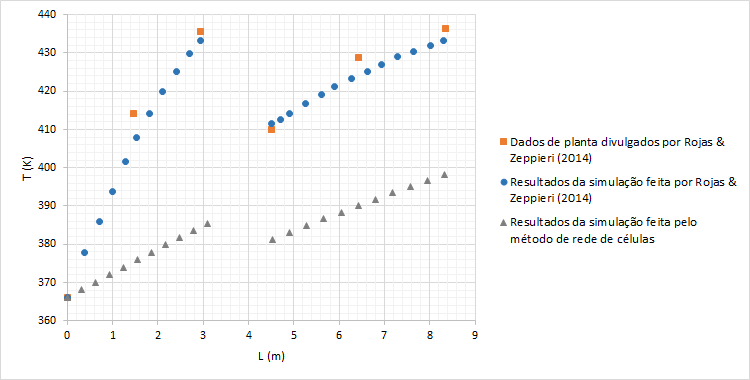
\includegraphics[scale=0.4]{images/Chap4/perfilTvalidacao.png}
\caption{Perfil de temperatura dos leitos.}
\label{fig:perfilTvalidacao}
\end{figure}

Duas questões precisam ser destacadas da \autoref{fig:perfilTvalidacao}.
A primeira delas refere-se a exortermia dos leitos catalíticos: a modelagem aqui
desenvolvida apresenta exortemia inferior aos demais dados. Esse fato, quando
analisado isoladamente, induz ao pensamento de que ou a simulação por rede de
células não fora bem equacionada ou a abordagem é inadequada para o sistema
estudado.

A segunda questão refere-se ao resfriamento na região zona de \emph{quench}. O
dado de planta apresenta um resfriamento de \SI{25.7}{K} entre os leitos
catalíticos; a simulação de \citeonline{Rojas2014a} apresenta resfriamento de
\SI{21,6}{K} para a região; e o valor encontrado no presente trabalho foi de
\SI{4,1}{K}. Essa situação torna-se mais enigmática ao se constatar que o
balanço de energia proposto por \citeonline{Rojas2014a} para a região de \emph{quench}
é ainda mais simplificado que o proposto neste estudo.

Uma análise do valor de LHSV (\emph{Liquid Hourly Space Velocity}) foi feita
na tentativa de trazer um esclarecimento às discrepâncias encontradas. O
parâmetro LHSV pode ser definido como: 
\begin{equation}
\textrm{LHSV} = F_{vol}^L/{V_{R}}
\label{eq:LHSV}
\end{equation}
onde $F_{v}^L$ é a vazão volumétrica em \si{m^3/h} de líquido e $V_{R}$ é o
volume total do reator (somados os dois leitos).

\nomenclature{$F_v$}{Vazão volumétrica \nomunit{m^3/h}}
\nomenclature[S]{$v$}{Referente ao volume}
\nomenclature{$V$}{Volume \nomunit{m^3}}
\nomenclature{$V_R$}{Volume total do reator \nomunit{m^3}}

A \autoref{tab:comparacaoLHSV} mostra alguns valores encontrados na literatura
para LHSV, incluindo o trabalho de \citeonline{Rojas2014a}.

\begin{table}[!htb]
\begin{center}
\caption{Comparação entre valores de LHSV calculados com base em dados
publicados na literatura.}
\label{tab:comparacaoLHSV}
\small
\begin{tabular}{lccc}
{Autor} & {$F_v^L$ (\si{m^3/h})} & {$V_R$ (\si{m^3})} &
{LHSV (\si{1/h})}
\\
\hline
{\citeonline{Arpornwichanop2008}} & 69 & 60 & 1.14 \\
{\citeonline{Mederos2007}} & 165 & 62 & 2.66 \\
{\citeonline{Rojas2014a}} & 347 & 18 & 19.76 \\
\bottomrule
\end{tabular}
\end{center}
\end{table}

!! Comparativamente fica claro que o valor de LHSV do trabalho de
\citeonline{Rojas2014a} está uma ordem de grandeza acima dos valores
comumente empregados nos projetos de reatores TBR. Infelizmente, as tentativas
de contato com os autores do trabalho de \citeonline{Rojas2014a} não lograram
exito até o momento. Sendo assim, não foi possível realizar a verificação dos
valores por eles publicados. !!

!! Sendo assim, foi necessário ajustar o valor da vazão de alimentação de
gasolina de pirólise para que os dados apresentassem coerência. O critério utilizado foi
o grau de resfriamento que ocorre na região de \emph{quench}. De maneira mais
direta, a vazão da carga conbinada (hidrogênio + \emph{pygas}) foi modificada
para que a diferença de temperatura entre a saída do primeiro leito e entrada do
segundo fossem semelhantes aos dados de planta e, também, aos demais dados
calculados por \citeonline{Rojas2014a}. Em outras palavras, a vazão de
carga do reator foi modificada (a menor) para ficar compatível com o valor da
corrente de \emph{quench}, adequando o grau de resfriamento na região de
\emph{quench} do reator. !!

Após várias tentativas, o valor de $F_{w,1}$ foi alterado para \SI{2,079e4}
{kg/h}. Com essa nova vazão, tanto o resfriamento da região de \emph{quench}
quando a exotermia dos leitos tornaram-se aderentes aos dados de planta e de
literatura, como está mostrado na \autoref{sec:estadoestacionario}.

A \autoref{tab:comparacaoLHSV2} repete os valores da
\autoref{tab:comparacaoLHSV}, mas agora com a inclusão do valor de LHSV
após o ajuste da vazão de carga do reator.

\begin{table}[!htb]
\begin{center}
\caption{Comparação entre LHSVs publicadas.}
\label{tab:comparacaoLHSV2}
\small
\begin{tabular}{lccc}
{Autor} & {$F_v^L$ (\si{m^3/h})} & {$V_R$ (\si{m^3})} &
{LHSV (\si{1/h})}
\\
\hline
{\citeonline{Arpornwichanop2008}} & 69 & 60 & 1.14 \\
{\citeonline{Mederos2007}} & 165 & 62 & 2.66 \\
{\citeonline{Rojas2014a}} & 347 & 18 & 19.76 \\
{Dados ajustados} & 76 & 18 & 4.34 \\
\bottomrule
\end{tabular}
\end{center}
\end{table}

\subsection{Determinação do Valor de $N_{Disc}$} \label{sec:determinacaoNDisc}

Nesta seção será apresentada a maneira como foi escolhido o valor ideal de
$N_{Disc}$. O valor escolhido foi utilizado em todas as simulações doravante
apresentadas.

A maneira mais simples (e talvez a mais adequada) de se determinar o número de
células é simular o reator com diferentes valores de $N_{Disc}$ e, então,
verificar os resultados de algumas variáveis chave. Duas variáveis
foram escolhidas: temperatura e fração molar global de hidrogênio.

A \autoref{fig:NDiscT} mostra o perfil de temperatura do leito superior, para
diferentes valores de $N_{Disc}$. Percebe-se que, entre $N_{Disc} = 4$ e
$N_{Disc} = 8$ ainda há alguma diferença no comportamento do perfil de
temperatura. Contudo, é imperceptível a diferença entre os perfis resultantes de
$N_{Disc} = 8$ e $N_{Disc} = 16$. 

\begin{figure}[htb] \centering
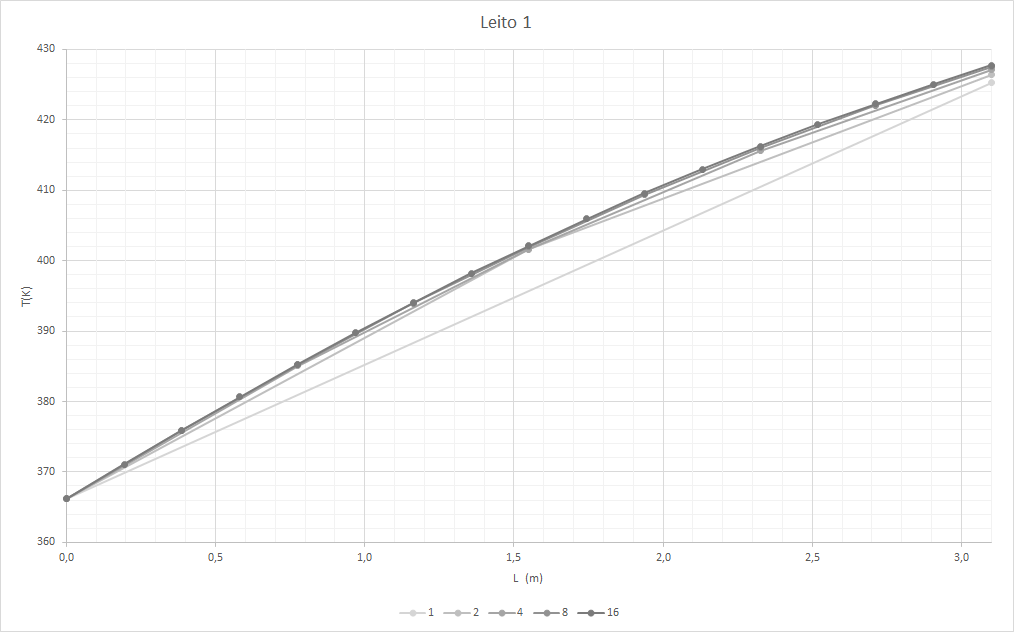
\includegraphics[scale=0.4]{images/Chap4/NDiscT.png}
\caption{Avaliação de NDisc pelo perfil de temperatura.}
\label{fig:NDiscT}
\end{figure}

Observando o perfil da fração molar global de hidrogênio de diferentes valores
de $N_{Disc}$ (também para o leito superior), é ainda menos relevante a
diferença entre $N_{Disc} = 4$ e $N_{Disc} = 8$, como mostra a
\autoref{fig:NDiscz}.

\begin{figure}[htb]
\centering 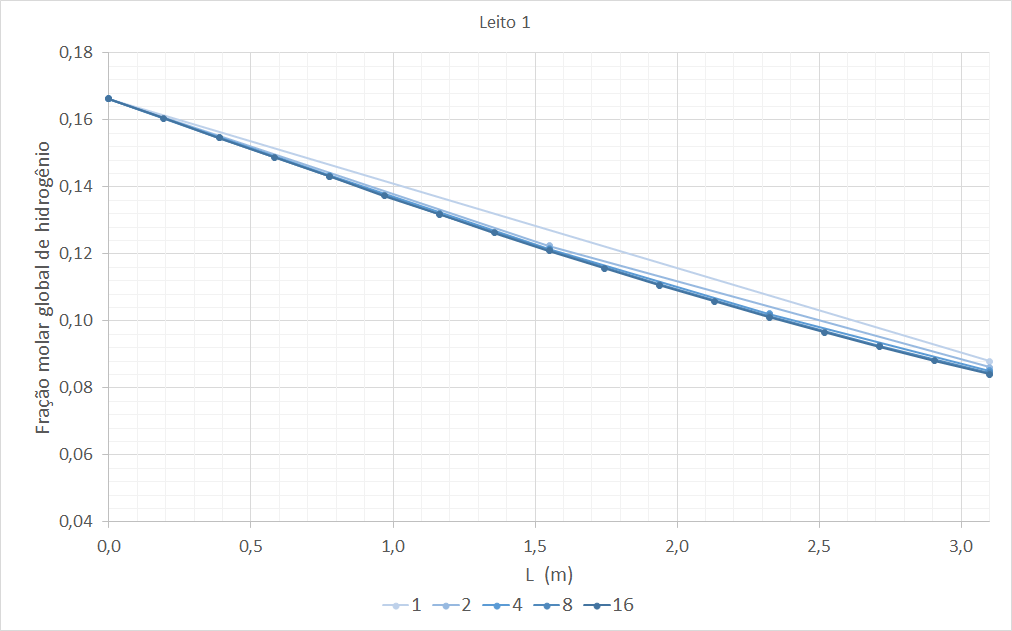
\includegraphics[scale=0.4]{images/Chap4/NDiscz.png}
\caption{Avaliação de NDisc pela fração molar total de hidrogênio.}
\label{fig:NDiscz}
\end{figure}

Assim, discretizar cada leito catalítico em $8$ células pareceria uma escolha
razoável e suficiente para o objetivo deste trabalho. Entretanto, para
garantir a representação dos leitos como contínuos, foi utilizado um valor um
pouco maior, $N_{Disc} = 10$. Esta escolha faz com que o modelo apresente um
total de $9299$ variáveis.

!! Mesmo não considerando a perda de carga nos resultados finais (como mostra a
\autoref{sec:avaliacaoperdadecarga}, as equações necessárias para os cálculos
dela foram mantidass. Além disso, algumas das equações hidrodinâmicas
influenciam em parâmetros de transferência de massa, que influenciam na taxa da
reação (Cs). Outras referem-se a avaliação do padrão de escoamento.  Dentro das
$9299$, portanto, estão todas as equações, mesmo as não relevantes para os
resultados. !!

\subsection{Avaliação da Perda de Carga} \label{sec:avaliacaoperdadecarga}

A equação da perda de carga quando implementada no modelo do reator causou
alguns problemas de convergência. Assim, optou-se primeiramente por avaliar a
importância da perda de carga, e se ela alteraria muito o perfil de pressão a
ponto de impactar no cálculo das propriedades das fases e do ELV.

Foi feita, portanto, uma simulação inicial que estimou a perda de carga, mas sem
alterar o perfil de pressão (pressão constante ao longo do reator). A perda de
carga estimada para os leitos está na \autoref{tab:perdadecarga}. Por esses
valores, percebe-se que a pressão ao longo dos leitos permanece praticamente
inalterada. Sendo assim, o reator foi simulado desprezando-se a perda de carga.

\begin{table}[!htb]
\begin{center}
\caption{Avaliação da perda de carga dos leitos.}
\label{tab:perdadecarga}
\small
\begin{tabular}{lccc}
{} & {$\Delta P/L$ (\si{atm/m})} & {Pressão de entrada (\si{atm})} & {Pressão de saída
(\si{atm})}
\\
\hline
{Leito 1} & \num{3.4e-3} & 49.64 & 49.63 \\
{Leito 2} & \num{3.7e-3} & 49.63 & 49.61 \\
\bottomrule
\end{tabular}
\end{center}
\end{table}

Um valor tão baixo assim de perda de carga não é o comumente encontrado na
indústria. Porém, a equação utilizada por \citeonline{Rojas2014a} e aqui neste
trabalho pode não ser a mais adequada, já que houve uma alteração da vazão de
carga do reator. Está mostrado na \autoref{sec:estadoestacionario} que o regime
de escoamento do reator se altera de regime de bolha (alta interação),
considerado por \citeonline{Rojas2014a}, para regime de escoamento gotejante
(baixa interação). Assim sendo, a equação para avaliação da perda de carga no
reator deveria ter sido outra mais adequada às características do sistema.

\section{Estado Estacionário} \label{sec:estadoestacionario}

\subsection{Perfil de Temperatura} \label{sec:perfildetemperatura}

A \autoref{fig:perfilT} mostra o perfil de temperatura dos leitos
calculado por este trabalho, além daquele calculado por \citeonline{Rojas2014a}
e pelos dados de planta por eles publicados.  

\begin{figure}[htb]
\centering 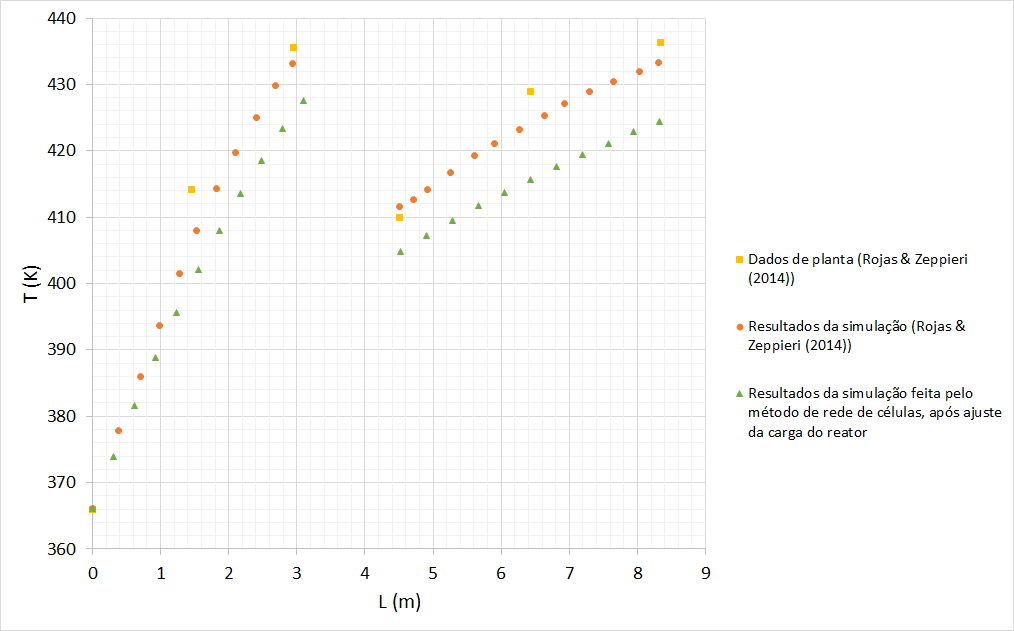
\includegraphics[width=0.8\textwidth]{images/Chap4/perfilT.png}
\caption{Perfil de temperatura dos leitos.}
\label{fig:perfilT}
\end{figure}

A diminuição drástica do valor da vazão de alimentação está refletida na alteração
do perfil de temperatura primeiramente encontrado
(\autoref{fig:perfilTvalidacao}). Sendo o perfil de temperatura obtido neste
trabalho semelhante tanto aos dados de planta quando aos valores calculados por
\citeonline{Rojas2014a}, é possível apresentar os demais resultados e efetuar
mais comparações.


\subsection{Composição da Corrente Efluente do Reator}
\label{composicaodacorrenteefluentedoreator}

\citeonline{Rojas2014a} divulgaram a composição do efluente do reator agrupando
alguns compostos. Assim sendo, foi implementado o mesmo agrupamento para fins de
comparação, como mostra a \autoref{tab:composicaodoefluente}. Pela comparação
entre os dados composicionais do efluente do reator, corrobora-se a opção de se
alterar a vazão de alimentação.

\begin{table}[!htb]
\begin{center}
\caption{Composição do Efluente do Reator em Fração Molar.}
\label{tab:composicaodoefluente}
\small
\begin{tabular}{lccc}
{Compostos} & {Dados de Planta} & {\citeonline{Rojas2014a}} & {Este Trabalho}
\\
\hline
{Hidrogênio} & 0.06 & 0.05 & 0.04 \\
{C1-C4 não reativos} & 0.05 & 0.04 & 0.04 \\
{C6-C9 não reativos} & 0.06 & 0.07 & 0.06 \\
{Benzeno-Tolueno-Xileno} & 0.48 & 0.47 & 0.48 \\
{Dienos C5-C6} & 0.00 & 0.00 & 0.00 \\
{Olefinas C5-C6} & 0.14 & 0.15 & 0.14 \\
{Parafinas C5-C6} & 0.10 & 0.12 & 0.14 \\
{Estirenos} & 0.00 & 0.00 & 0.00 \\
{Aromáticos reativos} & 0.06 & 0.07 & 0.07 \\
{Diciclodienos} & 0.00 & 0.00 & 0.00 \\
{Diciclodienos hidrogenados} & 0.03 & 0.03 & 0.03 \\
\bottomrule
\end{tabular}
\end{center}
\end{table}

\subsection{ELV} \label{elv}

Como está mencionado no \autoref{chap:moddesenvolvidos}, a fração de vapor
em cada célula $z$ é determinada por um cálculo de \emph{flash}, implementado no
modelo \code{streamTP}, detalhado no \autoref{chap:streamTP}. A
\autoref{fig:perfilfracaovaporizada} mostra o perfil da fração de vapor (base
molar) ao longo do leito catalítico.

\begin{figure}[htb]
\centering 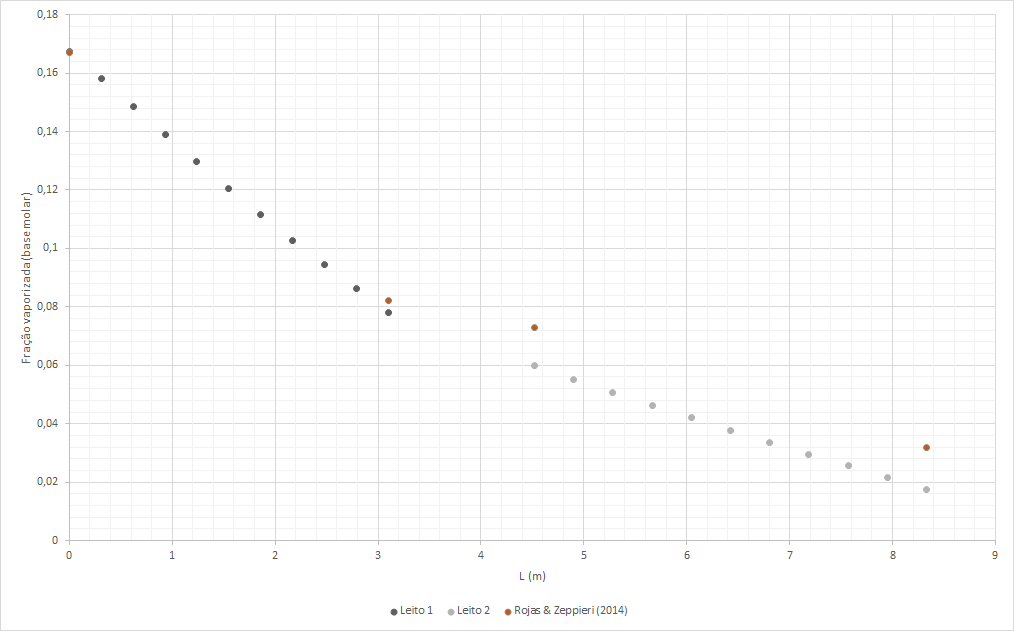
\includegraphics[scale=0.4]{images/Chap4/perfilfracaovaporizada.png}
\caption{Perfil de fração vaporizada.}
\label{fig:perfilfracaovaporizada}
\end{figure}

É possível perceber pela \autoref{fig:perfilfracaovaporizada} que a fração
vaporizada na entrada do primeiro leito calculada neste trabalho é muito próxima
daquela calculada por \citeonline{Rojas2014a}. Já para o segundo leito, há uma
diferença próxima a 20\% entre os dois conjuntos de resultados.

Duas questões entre o presente trabalho e o publicado por
\citeonline{Rojas2014a} podem justificar essa diferença.

A primeira delas é a questão da perda de carga. Neste trabalho, como explicado
na \autoref{sec:avaliacaoperdadecarga}, a perda de carga fora desprezada. Visto
que \citeonline{Rojas2014a} não publicaram o valor da perda de carga encontrada nos
leitos catalíticos, não é possível avaliar se há ou não uma influência da perda
de carga na fração vaporizada.

Há ainda outra diferença: o parâmetro de interação binaria $\delta_{ij}$ foi
calculada por \citeonline{Rojas2014a} utilizando a base de dados do software
comercial PRO/II 9.0. Ainda, a regra de mistura por eles apontada como a de melhor resultado (e,
entende-se como sendo a que foi utilizada para gerar os resultados publicados)
foi a de PA-RESimSci (SimSci-Esscor. PRO/II 9.0 Component and Thermophysical
Properties Reference Manual (2010)).

\subsection{Comportamento do Hidrogênio} \label{comportamentodohidrogenio}

Uma das premissas adotadas aqui, e que é oriunda do trabalho de
\citeonline{Rojas2014a}, é que a concentração de hidrogênio na
fase líquida é aproximadamente constante ao longo do reator. Por essa razão,
outra premissa também foi considerada, a de que as reações podem ser
consideradas como de pseudo-primeira ordem, desprezando a concentração de
hidrogênio.

!! A \autoref{fig:perfilfracaoh2liquido} confirma a premissa adotada, mostrando
que a fração molar de hidrogênio em fase líquida ao longo do reator não só é
praticamente constante, como também aumenta ao longo do reator. O aumento da
fração molar de hidrogênio na fase líquida é explicado pelo aumento da
tempeartura ao longo dos leitos, provocado pela liberação de calor das reações
de hidrogenação. A \autoref{fig:perfilfracaoh2temperatura} apresenta os
mesmos resultados de fração molar de hidrogênio na fase líquida
apresentados na \autoref{fig:perfilfracaoh2liquido}, mas desta vez referente à
temperatura de cada célula dos leitos do reator (relembrando que cada célula
\emph{z} tem uma temperatura e um comprimento atrelado a ela).
!!

\begin{figure}[htb]
\centering 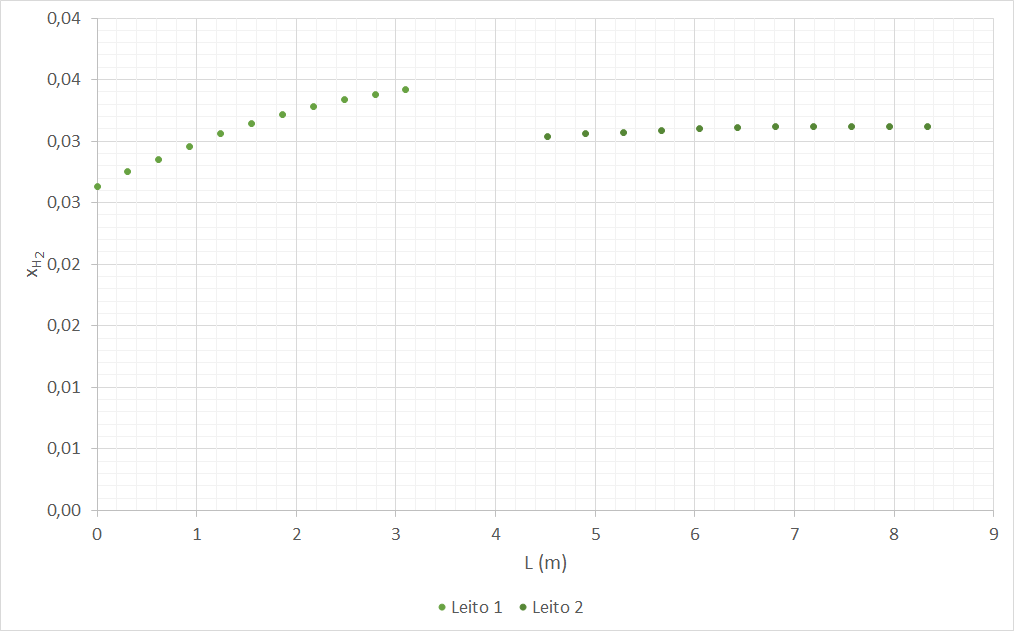
\includegraphics[scale=0.4]{images/Chap4/perfilfracaoh2liquido.png}
\caption{Perfil de fração molar de hidrogênio em fase líquida.}
\label{fig:perfilfracaoh2liquido}
\end{figure}

\begin{figure}[htb]
\centering
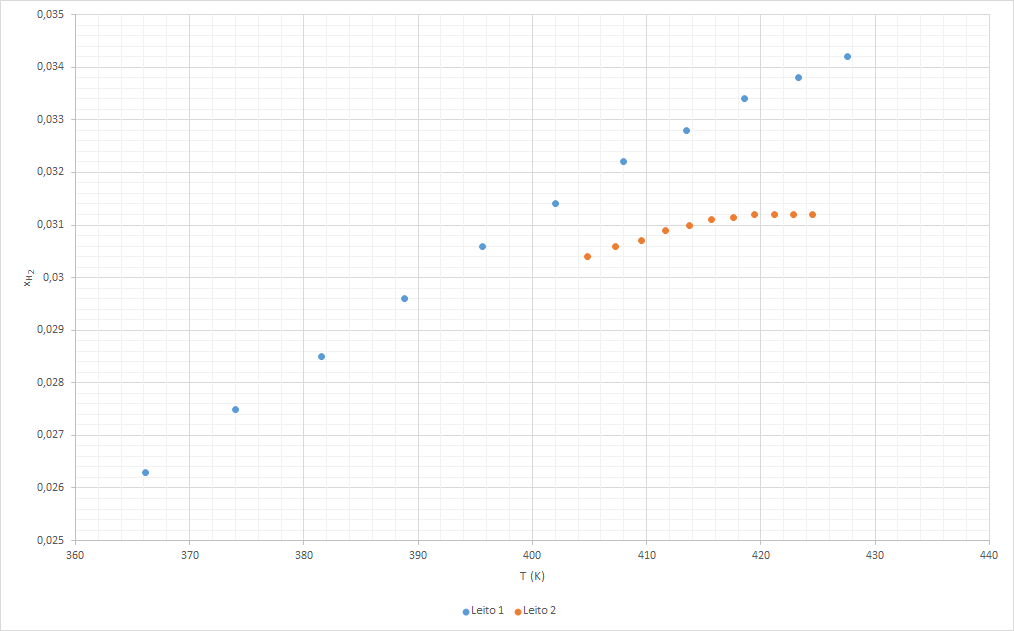
\includegraphics[scale=0.4]{images/Chap4/perfilfracaoh2temperatura.png}
\caption{Fração molar de hidrogênio em fase líquida \emph{vs.} da temperatura.}
\label{fig:perfilfracaoh2temperatura}
\end{figure}

A \autoref{fig:perfilfracaoh2gas} mostra o comportamento da
fração molar de hidrogênio na fase gasosa. Por ser consumido conforme as reações
avançam ao longo dos leitos catalíticos, o hidrogênio tende a diminuir de
concentração na fase gasosa ao longo do reator, como já era esperado.

\begin{figure}[htb]
\centering
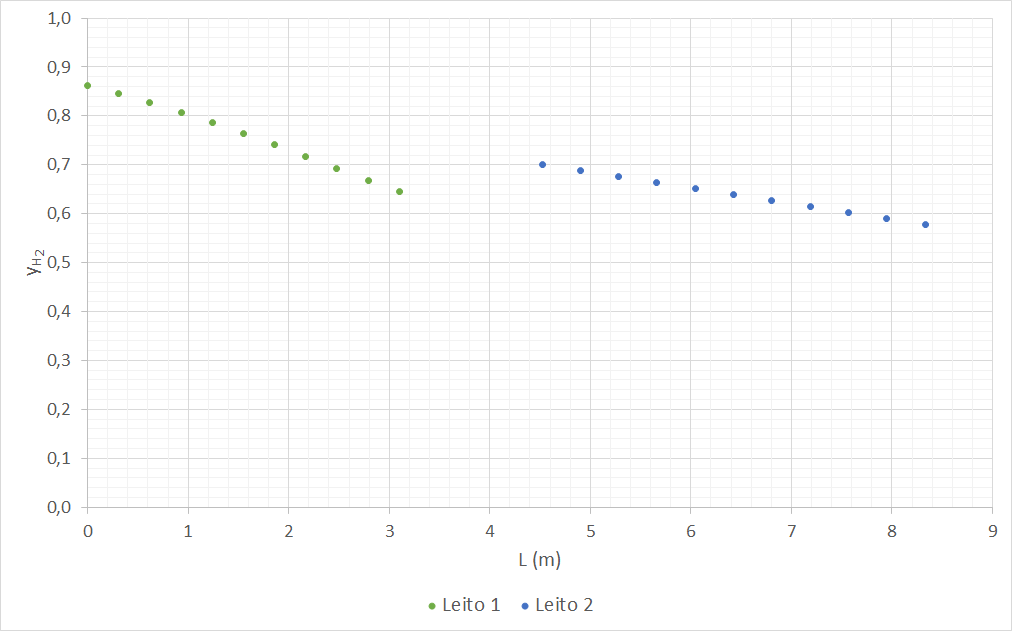
\includegraphics[scale=0.4]{images/Chap4/perfilfracaoh2gas.png}
\caption{Perfil de fração de hidrogênio em fase gasosa.}
\label{fig:perfilfracaoh2gas}
\end{figure}

\subsection{Propriedades Termodinâmicas} \label{propriedadestermodinâmicas}

A \autoref{tab:propriedadestermodinamicas} apresenta os valores de algumas
propriedades termodinâmicas calculadas neste trabalho.

\begin{table}[!htb]
\begin{center}
\caption{Propriedades Termodinâmicas.}
\label{tab:propriedadestermodinamicas}
\small
\begin{tabular}{lcccc}
{Propriedade} & {Entrada Leito 1} & {Saída Leito 1} & {Entrada Leito 2} &
{Saída Leito 2}
\\
\hline
{$MW^{L}$ (\si{kg/kmol})} & 82.5 & 81.6 & 81.6 & 81.2 \\
{$MW^{G}$ (\si{kg/kmol})} & 7.0 & 18.4 & 13.6 & 18.8 \\
{$\rho^{L}$(\si{kg/m^3})} & 728.7 & 639.9 & 668.9 & 635.3 \\
{$\rho^{G}$ (\si{kg/m^3})} & 11.4 & 26.4 & 20.3 & 27.2 \\
\bottomrule
\end{tabular}
\end{center}
\end{table}

!! Conforme já esperado, o resultado da simulação mostra que a densidade do
líquido diminui ao longo do primeiro leito catalítico (conforme há aumento de
temperatura), aumenta na região de \emph{quench} (devido à injeção de líquido
frio), e volta a diminuir ao longo do segundo leito. A densidade da fase gasosa
tem o comportamento inverso, já que mesmo com o aumento da temperatura, a
densidade da fase gasosa aumenta a medida que sua massa molar aumenta. !!

Mudança mais relevante sofre a massa molar da fase gasosa, que aumenta ao
longo do primeiro e segundo leitos, diminuindo na zona de \emph{quench}. Esse
comportamento é reflexo tanto da diminuição da concentração de hidrogênio na
fase gasosa, que tende a se diluir mais facilmente em fase líquida conforme a
temperatura aumenta, quanto da evaporação de compostos leves conforme o leito
catalítico aquece.

A massa molar do líquido tende a permanecer constante ao longo de todo o
reator, mostrando que o aumento da concentração de hidrogênio não é relevante
para alterar significativamente essa propriedade.

Os resultados das propriedades termodinâmicas parecem mais aderentes com
aqueles divulgados por \citeonline{Rojas2014a}. A diferença pode ser explicada
tanto por conta do pacote termodinâmico utilizado quanto pelo perfil de
temperatura resultante da simulação por eles realizada.

\subsection{Propriedades Hidrodinâmicas} \label{propriedadeshidrodinâmicas}

A \autoref{tab:propriedadeshidrodinamicas} mostra o resultado de algumas
propriedades hidrodinâmicas e números adimencionais utilizados nos cálculos de
transferência de massa e perda de carga.

\begin{table}[!htb]
\begin{center}
\caption{Propriedades Hidrodinâmicas.}
\label{tab:propriedadeshidrodinamicas}
\small
\begin{tabular}{lcccc}
{Propriedade} & {Entrada Leito 1} & {Saída Leito 1} & {Entrada Leito 2} &
{Saída Leito 2}
\\
\hline
{$u^{L}$ (\si{m/s})} & \num{3.2e-3} & \num{3,6e-3} & \num{4,7e-3} & \num{4,9e-3} \\
{$u^{G}$ (\si{m/s})} & \num{3,3e-3} & \num{1,7e-3} & \num{1,5E-3} & \num{0,5E-3} \\
{$\mu^{L}$(\si{cP})} & \num{0,128} & \num{0,103} & \num{0,130} & \num{0,121} \\
{$\mu^{G}$ (\si{cP})} & \num{0,012} & \num{0,013} & \num{0,012} & \num{0,013} \\
{$Re^{L}$} & \num{54,4} & \num{67,6} & \num{72,1} & \num{78,0} \\
{$Re^{G}$} & \num{10,6} & \num{10,1} & \num{7,6} & \num{3,0} \\
{$Ga^{L}$} & \num{8,6e6} & \num{10,4e6} & \num{7,0e6} & \num{7,4e6} \\
{$We^{L}$} & \num{1,5e-3} & \num{2,8e-3} & \num{4,1e-3} & \num{5,2e-3} \\
{$X^{G}$} & \num{7,8} & \num{2,3} & \num{1,8} & \num{0,5} \\
{$Pe^{L}$} & \num{428} & \num{443} & \num{600} & \num{609} \\
\bottomrule
\end{tabular}
\end{center}
\end{table}

É preciso informar aqui que os valores de $\mu^L$ e $\mu^G$ apresentados na
\autoref{tab:propriedadeshidrodinamicas} foram calculadas por rotinas internas
do simulador iiSE; os demais parâmetros foram calculados por equações
apresentadas na \autoref{chap:moddesenvolvidos}. Ademais, o comportamento da
viscosidade das fases foi como o esperado, ou seja, a viscosidade da fase
líquida diminui com o aumento da temperatura, e a viscosidade da fase gasosa
aumenta com o mesmo aumento (considerando que a pressão ao longo do reator é
constante).

Um resultado que chama a atenção na \autoref{tab:propriedadeshidrodinamicas}
refere-se à velocidade de escoamento das fases e, consequentemente, ao número de
Reynolds delas. A velocidade da fase líquida divulgada por
\citeonline{Rojas2014a}, por exemplo, esteve entre \SI{1,2e-2}{m/s} e
\SI{1,5e-2}{m/s}, o que é cerca de cinco vezes maior do que os valores
encontrados neste trabalho. Aqui, portanto, fica clara a divergência da vazão de
carga do reator utilizada neste trabalho e no trabalho original.

Os números de $Ga^L$ e $We^L$ foram usados para o cálculo de $\eta_{CE}$ e
$\epsilon^{L}$, respectivamente. Esses parâmetros estão apresentados nas seções
a seguir.

\subsubsection{Retenção Total de Líquido $\epsilon^{L}$}
\label{retencaototaldeliquido}

A \autoref{fig:perfilretencaoliquido} mostra o perfil da retenção de líquido
total $\epsilon^{L}$ ao longo dos leitos. Considerando que, ao longo do leito, a fração vaporizada diminui
(\autoref{tab:comparacaoLHSV2}), é coerente que a retenção de líquido aumente.
Do primeiro leito para o segundo leito há um aumento da retenção de líquido, que
é fruto do aumento da vazão de líquido dentro do reator causado pela injeção da
corrente líquida de \emph{quench}.

\begin{figure}[htb]
\centering
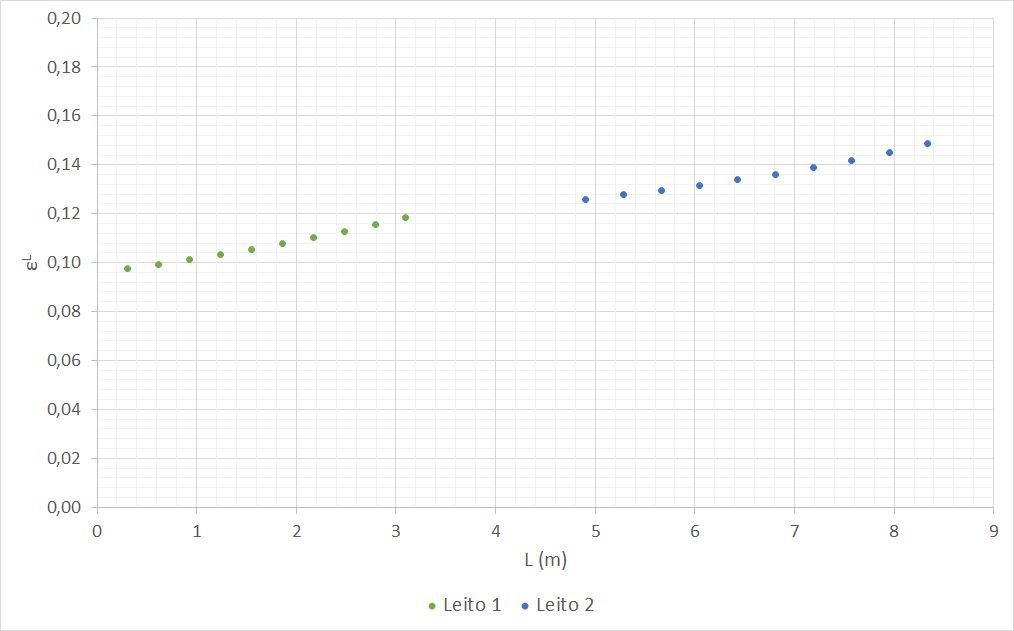
\includegraphics[scale=0.4]{images/Chap4/perfilretencaoliquido.png}
\caption{Perfil de $\epsilon^{L}$.}
\label{fig:perfilretencaoliquido}
\end{figure}

Como já explicado no \autoref{chap:moddesenvolvidos}, a variável $\epsilon^{L}$
possui como dimensão o valor de $N_{Disc}$.

Os valores $\epsilon^{L}$ encontrados por \citeonline{Rojas2014a} foram de
0,14 e 0,17 para a entrada do Leito 1 e saída do Leito 2,
respectivamente. A diferença entre os resultados pode ser explicada pela
incerteza quanto à vazão de carga no reator, que neste trabalho precisou ser
modificada por motivos já explicados. Contudo, a diferença não é tão
significativa assim, sendo ambos os trabalhos aderentes aos resultados de
literatura.

\subsubsection{Eficiência de Molhamento} \label{eficienciademolhamento}

A eficiência de molhamento $\eta_{CE}$ para o primeiro e o segundo leitos
catalíticos do reator aqui estudado foi estimada em \SI{0,72} e \SI{0,75},
respectivamente. Em seu trabalho, \citeonline{Rojas2014a} encontraram valores
maiores do que \SI{1,0} para o parâmetro $\eta_{CE}$.

Este é mais um caso onde a incerteza quanto à vazão de carga do reator
impossibilita uma análise comparativa mais acurada. De qualquer forma, vale a
observação de que, por possuir uma vazão de líquido maior devido a injeção da
corrente de \emph{quench}, o segundo leito do reator apresenta eficiêcia de
molhamento maior do que o primeiro, como já era esperado.

\subsubsection{Escoamento - Classificação} \label{escoamentoclassificacao}

Segundo \citeonline{Sie1998}, o regime de escoamento gotejante é definido
principalmente pelas velocidades superficiais das fases gás e líquida. Neste
trabalho há uma figura em que, de acordo com as velocidades superficiais das
fases, é possível verificar o tipo de escoamento no qual o reator opera. Segundo
essa figura, o reator estudado neste trabalho enquadra-se como um reator de
leito gotejante.

\citeonline{Saroha1996} publicaram um mapa mais elaborado que classifica o
escoamento dos reatores trifásicos de leito fixo. De acordo com esse mapa, os
valores encontrados na presente simulação colocam o reator objeto de estudo na
região de escoamento tipo leito gotejante.

Assim, o tipo de escomento encontrado aqui para o reator é contrário à premissa
adotada de escoamento tipo bolha. É preciso lembrar que este trabalho
preocupou-se em manter ao máximo as premissas e valores publicados por
\citeonline{Rojas2014a}. Contudo, a premissa adotada para o tipo de escoamento
(borbulhamento), que influencia na escolha das equações hidrodinâmicas, deveria
ser revista e outras equações hidrodinâmicas deveriam ter sido utilizadas no
lugar das atuais.

\subsection{Transferência de Massa - Interface Líquido-Sólido}
\label{transferênciademassainterfaceliquidosolido}

Como assumido nas premissas deste trabalho, a transferência de massa entre as
fases gasosa e líquida foi desprezada, ficando então a composição \emph{bulk}
destas fases definida pelo ELV.

Já a composição dos reagentes e produtos na superfície do catalisador ($C^S$)
foi considerada distinta da composição \emph{bulk} da fase líquida $C^L$. A
\autoref{tab:concentraçõesparaoleito1} mostra as concentrações dos compostos na
fase líquida (\emph{bulk}) e na superfície do catalisador para a entrada e a
saída do Leito 1. De acordo com os resultados, fica evidente que a diferença dos
valores de $C^S$ e $C^L$ para cada um dos compostos é mínima.

Assim, a taxa da reação poderia muito bem ser calculada com a composição
\emph{bulk} da fase líquida $C^L$, desprezando-se a transferência de massa na
interface líquido-sólido.

\begin{table}[!htb]
\begin{center}
\caption{Concentrações $C^L_{i}$ e $C^S_{i}$ para o Leito 1.}
\label{tab:concentraçõesparaoleito1}
\small
\begin{tabular}{lcccc}
{Composto} & {$C^{L}_{1}$} & {$C^{S}_{1}$} & {$C^{L}_{11}$} & {$C^{S}_{11}$}
\\
\hline
{Hidrogênio} & 0.2397 & 0.2367 & 0.2656 & 0.2644 \\
{Metano} & 0.1002 & 0.1002 & 0.1304 & 0.1304 \\
{Etano} & 0.0210 & 0.0210 & 0.0208 & 0.0208 \\
{n-Propano} & 0.0511 & 0.0511 & 0.0468 & 0.0468 \\
{n-Butano} & 0.0352 & 0.0352 & 0.0312 & 0.0312 \\
{n-Pentano} & 0.5327 & 0.5328 & 0.5070 & 0.5073 \\
{trans-2-Penteno} & 0.5512 & 0.5519 & 0.5876 & 0.5879 \\
{trans-1.3-Pentadieno} & 0.2455 & 0.2447 & 0.0739 & 0.0734 \\
{Ciclopentano} & 0.1557 & 0.1559 & 0.1911 & 0.1914 \\
{Ciclopenteno} & 0.2539 & 0.2554 & 0.3054 & 0.3053 \\
{Metil-1.3-Ciclopentadieno} & 0.1611 & 0.0210 & 0.0208 & 0.0208 \\
{n-Hexano} & 0.2757 & 0.2757 & 0.2424 & 0.2424 \\
{Metilciclopentano} & 0.1383 & 0.1383 & 0.1370 & 0.1371 \\
{Metilciclopenteno} & 0.1866 & 0.1871 & 0.2428 & 0.2430 \\
{1.3-Ciclopentadieno} & 0.1695 & 0.1680 & 0.0128 & 0.0126 \\
{Benzeno} & 2.6803 & 2.6803 & 2.3579 & 2.3579 \\
{n-Heptano} & 0.2029 & 0.2029 & 0.1786 & 0.1786 \\
{Tolueno} & 1.2642 & 1.2642 & 1.1141 & 1.1141 \\
{n-Octano} & 0.0825 & 0.0825 & 0.0727 & 0.0727 \\
{Etilbenzeno} & 0.2536 & 0.2546 & 0.3146 & 0.3148 \\
{Estireno} & 0.1207 & 0.1197 & 0.0156 & 0.0155 \\
{Xileno} & 0.3712 & 0.3712 & 0.3277 & 0.3277 \\
{n-Nonano} & 0.0376 & 0.0376 & 0.0332 & 0.0332 \\
{1-Metil-3-Etilbenzeno} & 0.1813 & 0.1816 & 0.2081 & 0.2083 \\
{Metilestireno} & 0.0813 & 0.0810 & 0.0239 & 0.0237 \\
{Dihidrodiciclopentadieno} & 0.2003 & 0.2014 & 0.2721 & 0.2724 \\
{Diciclopentadieno} & 0.1262 & 0.1251 & 0.0164 & 0.0161 \\
\bottomrule
\end{tabular}
\end{center}
\end{table}

\section{Respostas Dinâmicas} \label{sec:respostasdinamicas}
!!
A simulação concebida neste trabalho nasceu preparada para estudos e avaliações
de respostas dinâmicas. Quatro avaliações de respostas dinâmicas foram feitas, a
saber:

\begin{enumerate}
  \item Resposta a   um degrau na temperatura da carga, de \SI{366}{K} para
  \SI{300}{K} - Avaliação da importância da inércia térmica do catalisador;
  \item Resposta a um degrau na vazão da corrente de quench, de \SI{20790}{kg/h}
  para \SI{10790}{kg/h}; e
  \item Resposta a um degrau na vazão da corrente de quench, de \SI{20790}{kg/h}
  para \SI{30790}{kg/h}.
\end{enumerate}

As seções a seguir apresentam uma breve discussão para cada um dos casos
mencionados.

\subsection{Resposta a   um degrau na temperatura da carga, de \SI{366}{K} para
\SI{300}{K} - Avaliação da importância da inércia térmica do catalisador}
\label{sec:respostaaumdegrautemp}

Este primeiro caso reflete o comportamento do reator no caso da perda de
aquecimento da carga, seja por falta de utilidades (vapor para um trocador de
calor, por exemplo), seja por falha nos elementos primários de uma eventual
malha de controle. Como consequência dessa perda de aquecimento da carga, o
exotermia vista em operação normal diminui drasticamente, sinal de que a
conversão dos reagentes passou a patamares inaceitáveis. O perfil de temperatura
dos leitos do reator após o degrau de temperatura na carga está mostrado na
\autoref{fig:Feed_T_300K}.

\begin{figure}[htb]
\centering
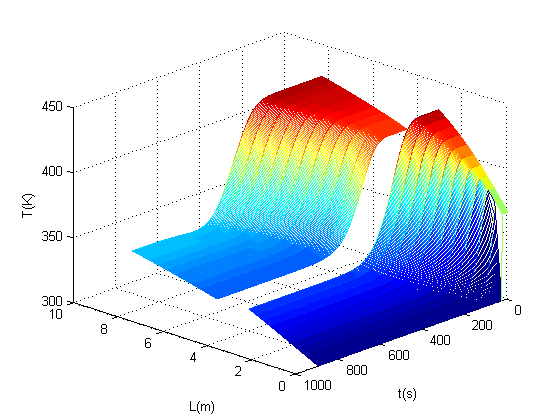
\includegraphics[scale=0.8]{images/Chap4/Feed_T_300K.png}
\caption{Resposta dinâmica do perfil de tempeartura a um degrau (a menor) de
temperatura na carga.}
\label{fig:Feed_T_300K}
\end{figure}

A \autoref{fig:Feed_T_300K} não considera a influência do catalisador na inércia
térmica, i.e., considera a \autoref{eq:holdupenergia} para o cálculo da energia
acumulada em cada célula. Dessa forma, o tempo até o reator atingir o novo
estado estacionário após o degrau foi de aproximadamente \si{900}{s}.

Ao ser calculada a energia acumulada em cada célula pela
\autoref{eq:holdupenergiadinamica}, que considera a presença do catalisador, o
tempo para se atingir o novo estado estacionário passou a ser de aproximadamente
\si{3000}{s}! A \autoref{fig:Feed_T_300K_catalyst_influence} mostra o perfil de
temperatura dos leitos do reator após o degrau de temperatura na carga,
considerando a inércia térmica do catalisador.

\begin{figure}[htb]
\centering
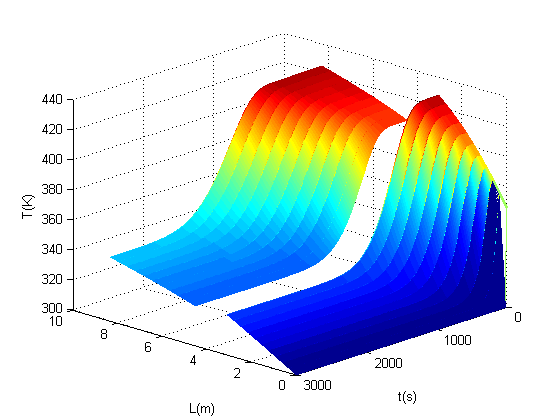
\includegraphics[scale=0.8]{images/Chap4/Feed_T_300K_catalyst_influence.png}
\caption{Resposta dinâmica do perfil de tempeartura a um degrau (a menor) de
temperatura na carga, considerando a inércia térmica do catalisador}
\label{fig:Feed_T_300K_catalyst_influence}
\end{figure}

% A concentração de diolefinas na saída do reator passa de \si{0.0305}{kmol/m^3}
% para \si{0.2868}{kmol/m^3}; 
% 
% \begin{figure}[htb]
% \centering
% 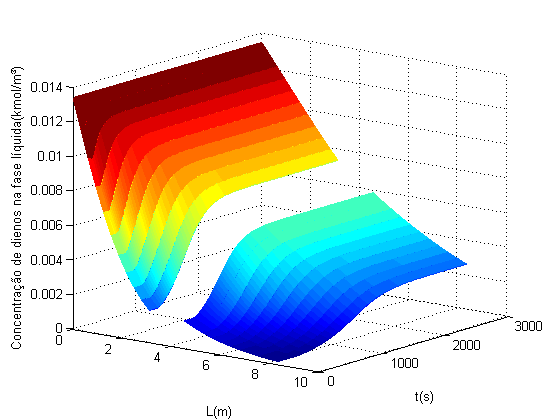
\includegraphics[scale=0.8]{images/Chap4/Feed_T_300K_catalyst_influence_dienes.png}
% \caption{Resposta dinâmica da concentração de diolefinas a um degrau (a menor)
% de temperatura na carga.}
% \label{fig:Feed_T_300K_catalyst_influence_dienes}
% \end{figure}

Além do perfil de temperatura, vale aqui apresentar o efeito do resfriamento da
carga do reator na concentração de estireno. A diminuição da temperatura de
entrada faz com que a fração molar total de estireno na saída do reator aumente
de \si{1.96e-4}{} para \si{0.0026}{}, cerca de $13.3$ vezes maior. Considerando
que o estireno é um composto que precisa ser eliminado da nafta de pirólise, a
queda de temperatura em questão é inaceitável. A
\autoref{fig:Feed_T_300K_catalyst_influence_styrene} mostra como seria a
resposta dinâmica do perfil da concentração de estireno ao degrau de temperatura
(a menor) da carga.

\begin{figure}[htb]
\centering
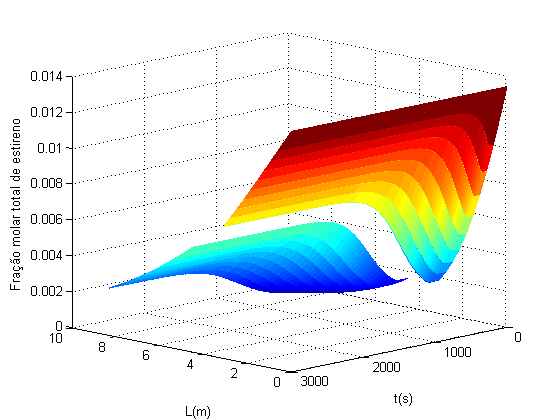
\includegraphics[scale=0.8]{images/Chap4/Feed_T_300K_catalyst_influence_styrene.png}
\caption{Resposta dinâmica da concentração de estireno um degrau (a menor) de
temperatura na carga.}
\label{fig:Feed_T_300K_catalyst_influence_styrene}
\end{figure}

As duas próximas avaliações de respostas dinâmicas foram feitas considerando o
catalisador no cálculo da energia acumulada nas células.

\subsection{Resposta a um degrau na vazão da corrente de \emph{quench}, de 20790
kg h para 10790 kg} \label{sec:respostaaumdegrauvazao1}

A perda de parte da vazão da corrente de \emph{quench} tem efeito imediato no
Leito 2 do reator, como mostra a \autoref{fig:Quench_F_10790_catalyst_influence}.

\begin{figure}[htb]
\centering
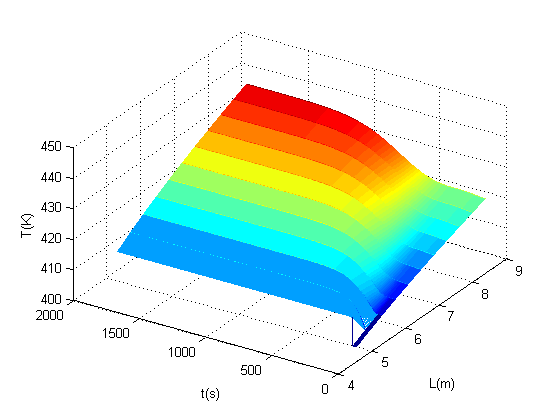
\includegraphics[scale=0.8]{images/Chap4/Quench_F_10790_catalyst_influence.png}
\caption{Resposta dinâmica a um degrau (a menor) na vazão de \emph{quench}.}
\label{fig:Quench_F_10790_catalyst_influence}
\end{figure}

É importante notar aqui que a perda parcial da vazão de \emph{quench} poderia
levar algumas regiões do reator a temperaturas altas o suficiente para causar
disparos de temperatura. De qualquer forma, a exotermia observada significa
também maior conversão de olefinas que, para o objetivo desse processo (produzir
gasolina automotiva), tem efeito deletério quanto à octanagem.

\subsection{Resposta a um degrau na vazão da corrente de \emph{quench}, de 20790
kg h para 30790 kg} \label{sec:respostaaumdegrauvazao3}

Para a situação em que a vazão da corrente de \emph{quench} aumenta, quer seja
por problema de instrumentação ou equipameto, quer seja por erro humano, o Leito
2 é esfriado como mostra a Figura \autoref{fig:Quench_F_30790_catalyst_influence}.

\begin{figure}[htb]
\centering
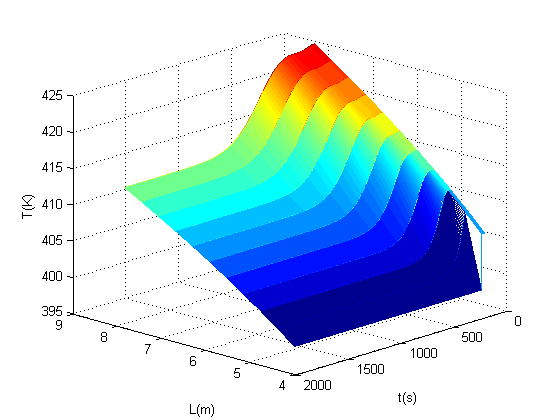
\includegraphics[scale=0.8]{images/Chap4/Quench_F_30790_catalyst_influence.png}
\caption{Resposta dinâmica a um degrau (a maior) na vazão de \emph{quench}.}
\label{fig:Quench_F_30790_catalyst_influence}
\end{figure}

Um problema neste caso é a queda na conversão dos compostos diolefínicos, o
que conferiria uma característica instável à gasolina automotiva.